\chapter{Valid Outcomes of Positive Support Size Five}

\section{Hexagon Criterion}

We introduce the \emph{Hexagon Criterion}, first presented in \cite{bik2022classifying}, to determine whether subconfigurations of a chipsplitting outcome qualify as outcomes. This criterion applies to configurations supported within the yellow area below; we say the support is not contained inside the ``hexagon".

\begin{figure}[H]
    \centering
    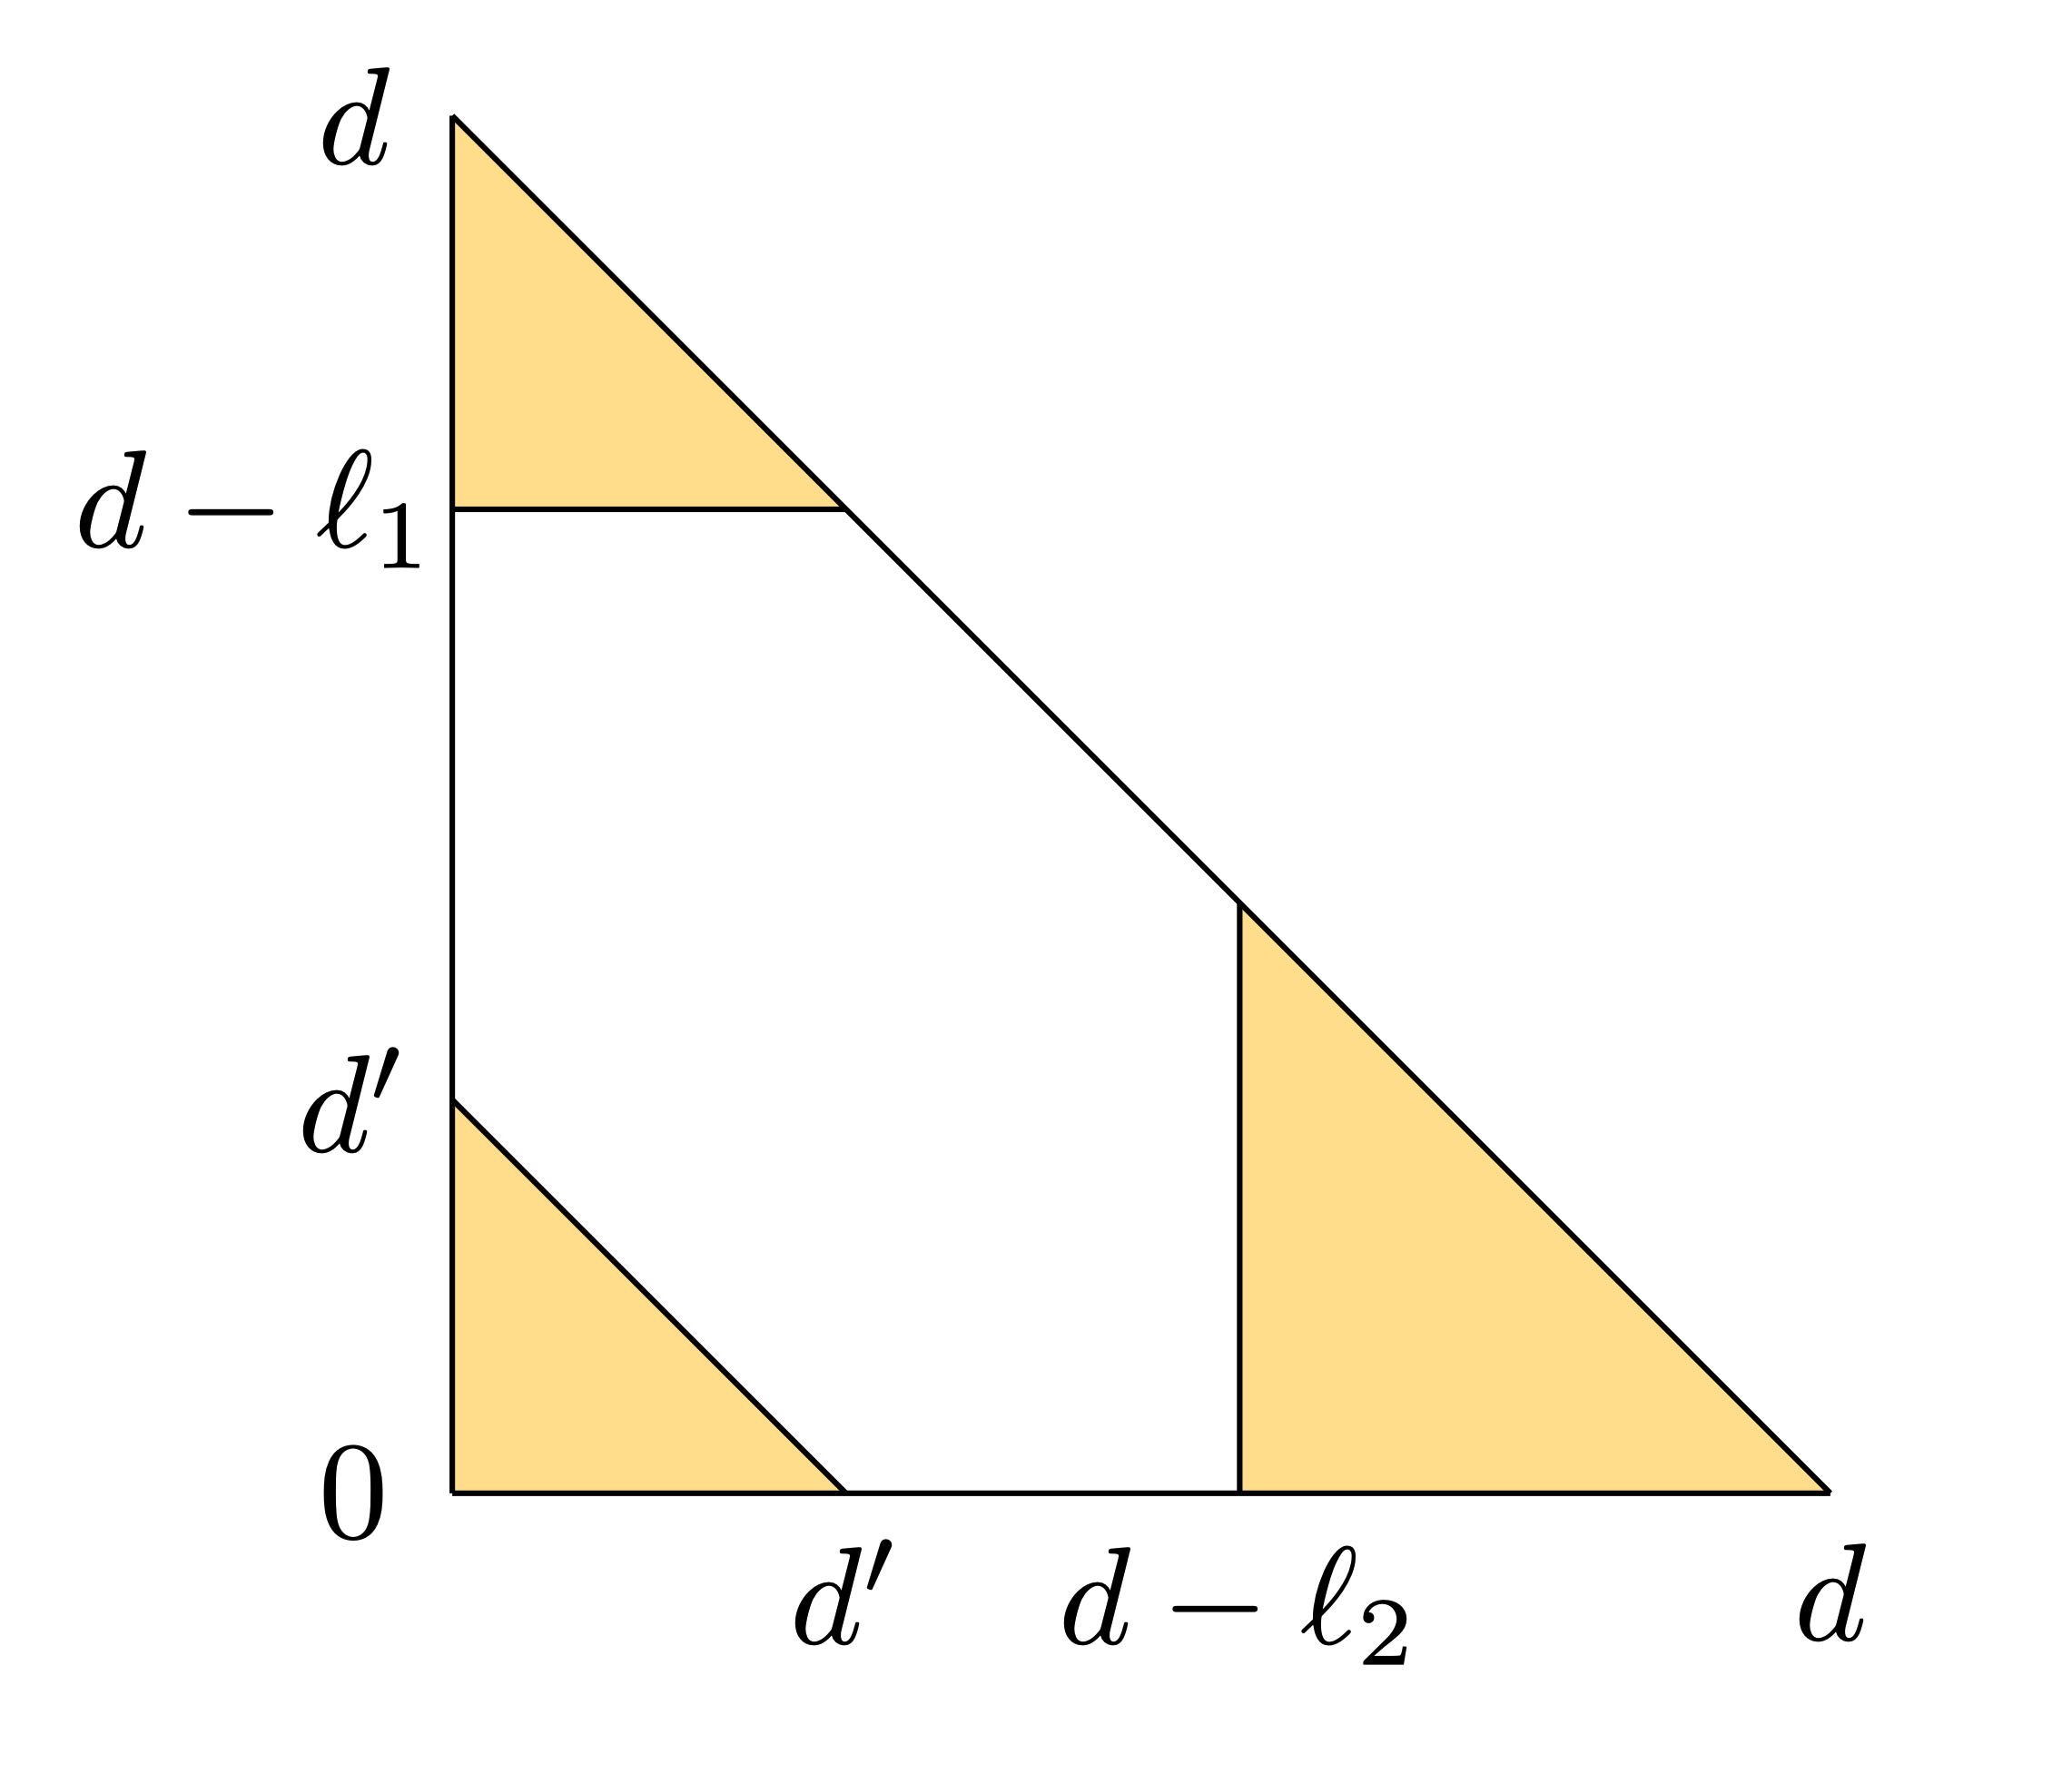
\includegraphics[width=0.5\textwidth]{assets/hexagon.png}
    \caption{A configuration's support lies outside the hexagon if it is contained in the yellow area spanned by parameters \( \ell_1, \ell_2 \), and \( d' \).}     \label{fig:hexagon}
\end{figure}

First, we need the following lemma to compute the determinant of matrix that we will encounter in the proof of the Hexagon Criterion.

\begin{lemma}\label{lemma:grinberghyperfactorial}
    Let \( a,b,c \in \mathbb{Z}_{\geq 0} \). Define the map \( H:  \mathbb{Z}_{\geq 0} \to  \mathbb{Z}_{\geq 0}, n \mapsto 0! 1! \cdots (n-1)! \); note that \( H(0) = 1 \). Then, the following holds:
    \begin{align*}
        \mathrm{det}\left(\begin{bmatrix}
            \binom{a+b}{b-i+j}
        \end{bmatrix}_{i,j = 1}^c\right) = \frac{H(a)H(b)H(c)H(a+b+c)}{H(b+c)H(c+a)H(a+b)}.
    \end{align*} 
\end{lemma}

\begin{proof}
    See Theorem 8 of \cite{grinberghyperfactorial}.
\end{proof}

We state the Hexagon Criterion.

\begin{proposition}\label{prop:hexagon-criterion231312}
    Let \( d, d', \ell_1, \ell_2 \in \mathbb{N} \) with \( d' \geq 1 \), \( \ell_1, \ell_2 \geq d' \), and \( d' + \ell_1 + \ell_2 \leq d \). Let \( \mathbf{w} = (w_{i,j})_{(i,j) \in V_d} \in \mathbb{Z}^{V_d} \) be a chip configuration. Define the subconfiguration \( \mathbf{w}' \coloneqq (w_{i,j})_{(i,j) \in V_{d'}} \in \mathbb{Z}^{V_{d'}}\). Assume the support of \( \mathbf{w} \) is not contained inside the ``hexagon" (see Figure \ref{fig:hexagon}), i.e. \( \mathrm{supp}(\mathbf{w}) \subset V_{d'}  \cup \left\{ (i,j) \in V_d \mid j > d - \ell_1 \right\} \cup \left\{ (i,j) \in V_d \mid i > d - \ell_2 \right\} \).
    Then, the following holds:
    \begin{enumerate}
        \item If \( \mathbf{w} \) is an outcome, then also its subconfiguration \( \mathbf{w}' \) is an outcome.
        \item If \( \mathbf{w} \) is a valid outcome, then \( \mathrm{deg}(\mathbf{w}) \leq d' \).
    \end{enumerate}
\end{proposition}

\begin{proof}
    We prove the first statement. Assume \( \mathbf{w} \) is an outcome. Let \( k = 0, \dots, d' \) and \( \mathrm{diag}(\ell_1 + k) = \sum_{(i,j) \in V_d} \mu_{i,j} x_{i,j} \). Consider the restricted linear form \( l_k = \sum_{(i,j) \in V_{d'}} \lambda_{i,j}x_{i,j} : \mathbb{Z}^{V_{d'}} \to \mathbb{Z} \) with \( \lambda_{i,j} \coloneqq \mu_{i,j} \) for \( (i,j) \in V_{d'} \). Then, \( l_0, \dots, l_{d'} \) are Pascal forms on \( \mathbb{Z}^{V_{d'}} \) with \( l_k(\mathbf{w}') = \mathrm{diag}(\ell_1 + k)(\mathbf{w}) = 0 \). By Proposition \ref{thm:pascal-outcome} it suffices to show that \( l_0, \dots, l_{d'} \) are linearly independent to show that \( \mathbf{w}' \) is an outcome.

    Let \( a = 0, \dots, d' \). Define
    \begin{align*}
        e_{{i,j}}^{(a)} &\coloneqq \begin{cases}
            1 & \text{ if } i = a \text{ and } j = d' - a, \\
            0 & \text{ otherwise}.
        \end{cases}\\
        A &\coloneqq \begin{bmatrix}
            l_k(\mathbf{e}^{(a)})
        \end{bmatrix}^{d'}_{k,a = 0} = \begin{bmatrix}
            \binom{d-d'}{\ell_1 + k - a}
        \end{bmatrix}^{d'}_{k,a = 0} = \begin{bmatrix}
            \binom{(d-d' - \ell_1) + \ell_1}{\ell_1 + k - a}
        \end{bmatrix}^{d'}_{k,a = 0}.
    \end{align*}
    We want to show that the matrix \( A \) is invertible because this implies that the linear forms \( l_0, \dots, l_{d'} \) are linearly independent. We observe that 
    \begin{enumerate}
        \item all entries of \( A \) are nonzero because \( 0 \leq \ell_1 + k - a \leq d - d' \), and 
        \item \( d - d' - \ell_1 \geq \ell_2 \geq 0 \).
    \end{enumerate}
    This allows us to use Lemma \ref{lemma:grinberghyperfactorial} with \( a \coloneqq d - d' - \ell_1, b \coloneqq \ell_1\), and \( c \coloneqq d' + 1 \).
    We obtain a nonzero determinant \( \mathrm{det}(A) = \frac{H(d - d' - \ell_1)H(\ell_1)H(d' + 1)H(d+1)}{H(\ell_1 + d' + 1)H(1 + d - \ell_1)H(d - d')} \neq 0 \).
    Hence, \( l_0, \dots, l_{d'} \) are linearly independent.

    For the second statement, let \( \mathbf{w} \) be a valid outcome. By the previous statement, the subconfiguration \( \mathbf{w}' \) is an outcome, as well. We extend \( \mathbf{w}' \) to some configuration \( \mathbf{v} \in \mathbb{Z}^{V_d} \) by \( v_{i,j} \coloneqq \begin{cases}
        w_{i,j}' & \text{ if } (i,j) \in V_{d'}, \\
        0 & \text{ otherwise}
    \end{cases} \).
    Clearly, \( \mathbf{v} \) is a \emph{valid} outcome of degree at most \( d' \). Then, \( \mathbf{v} - \mathbf{w} \) is an outcome with empty negative support. By Proposition \ref{prop:outcome-zero}, \(  \mathbf{v} - \mathbf{w} \) is zero. Hence, \( \mathrm{deg}(\mathbf{w}) \leq d' \).
\end{proof}



Next, we prove that for all valid integral outcomes \( \mathbf w \) with \( |\mathrm{supp}^+(\mathbf w)| = 5 \) we have \( \mathrm{deg}(\mathbf w) \leq 7 \). We use the Invertibility Criterion, Hyperfield Criterion, and the Hexagon Criterion.

\section{Proof \( d = 8, \dots, 41 \)}

First, we show that no outcome of degree \( d = 8, \dots, 41 \) exists with \( |\mathrm{supp}^+(\mathbf w)| = 5 \); this is similar to the proof of Proposition \ref{prop:jdngkjrenj3nw}.


\begin{proposition}\label{prop:uiwuwinca}
    No outcome of degree \( d = 8, \dots, 41 \) exists with \( |\mathrm{supp}^+(\mathbf w)| = 5 \).
\end{proposition}

\begin{proof}
    Let \( d = 8, \dots, 41 \). We define the system $A = \{ \mathrm{diag}(i) \}_{i=0}^d \cup \{ \mathrm{row}(i)\}^d_{i=0} \cup \{ \mathrm{col}(i) \}^d_{i=0}$. Then, we compute the set \( S_5(A) \) using Algorithm \ref{alg:solve}. Next, we apply Algorithm \ref{alg:hyperfield_criterion:is_zero} to each \( \mathbf{s} \in S_5(A) \). The implementation is found in \cite{ducrepo} under \texttt{chapter06.ipynb}.
\end{proof}

\section{Proof \( d \geq 42 \)}

We show that no valid outcome of degree \( d \geq 42 \) exists using contractions. As in Proposition \ref{prop:jasndkjsnjsnkjs}, we compute the sets \(  \Gamma^{\mathrm{even}} \cap \left\{ \mathbf{s} \in H^{\Xi} : \lvert \mathrm{supp}^+(\mathbf{s}) \rvert \leq 5 \right\} \) and \( \Gamma^{\mathrm{odd}} \cap \left\{ \mathbf{s} \in H^{\Xi} : \lvert \mathrm{supp}^+(\mathbf{s}) \rvert \leq 5 \right\}  \)
using Algorithm \ref{alg:hyperfield_criterion:efficient}. By Proposition \ref{prop:jasndkjsnjsnkjs}, we just need to check the case \( \lvert \mathrm{supp}^+(\mathbf{s}) \rvert = 5 \).



\begin{definition}
    We define the sets \( \Gamma^{\mathrm{even}}_5 \coloneqq \Gamma^{\mathrm{even}} \cap \left\{ \mathbf{s} \in H^{\Xi} : \lvert \mathrm{supp}^+(\mathbf{s}) \rvert = 5 \right\} \) and \( \Gamma^{\mathrm{odd}}_5 \coloneqq \Gamma^{\mathrm{odd}} \cap \left\{ \mathbf{s} \in H^{\Xi} : \lvert \mathrm{supp}^+(\mathbf{s}) \rvert = 5 \right\} \).
\end{definition}

\begin{proposition}
    We have \( \lvert \Gamma^{\mathrm{even}}_5 \rvert  = 1283\) and \( \lvert \Gamma^{\mathrm{odd}}_5 \rvert  = 1265\).
\end{proposition}

\begin{proof}
    This is verified by computer; see \cite{ducrepo}, specifically the file \texttt{chapter06.ipynb}.
\end{proof}

\begin{corollary}
    Let \( d\geq 42 \). Let \( \mathbf{w} \in \mathbb{Z}^{V_d} \) be a valid outcome of degree \( d \) with \( |\mathrm{supp}^+(\mathbf w)| = 5 \). Then, \( \mathrm{contr}_d(\mathrm{sign}(\mathbf{w})) \in \Gamma^{\mathrm{even}}_5 \cup \Gamma^{\mathrm{odd}}_5 \).
\end{corollary}

\begin{proof}
    This follows from Corollary \ref{cor:validwunfwufneuiw}.
\end{proof}

For each \( \mathbf{s} \in \Gamma^{\mathrm{even}}_5 \cup \Gamma^{\mathrm{odd}}_5 \), we want to show that any valid outcome \( \mathbf{w} \in \mathbb{Z}^{V_d} \) that maps to \( \mathbf{s} \) under \( \mathrm{contr}_d \circ \mathrm{sign} \) is the initial configuration. Note that \( \lvert \Gamma^{\mathrm{even}}_5 \cup \Gamma^{\mathrm{odd}}_5 \rvert = 2318 \); so we have to check \( 2318 \) cases. To make life easier when checking these cases, we simplify the index set \( \Xi \).

\begin{definition}
    Define the index set 
    \begin{align*}
        \Xi' \coloneqq \left\{ 0,1,2,3 \right\}^2 \sqcup \left\{ 0,1,2,3 \right\}^2 \sqcup \left\{ 0,1,2,3 \right\}^2 \sqcup \left\{ 0,1,2,3 \right\} \sqcup \left\{ 0,1,2,3 \right\} \sqcup \left\{ 0,1,2,3 \right\} 
    \end{align*}
    with the map \( \chi: H^\Xi \to H^{\Xi'}\) defined by \(  \mathbf{s} = (\mathbf{x}, \mathbf{y}, \mathbf{z}, \mathbf{b}, \mathbf{c}, \mathbf{d}, \mathbf{e}) \mapsto (\mathbf{x}, \mathbf{y}, \mathbf{z}, \mathbf{b}, \mathbf{c}, \underbracket{\mathbf{d} + \mathbf{e}}_{\coloneqq \mathbf{f}}) \).
    The new coordinate system \( H^{\Xi'} \) is depicted below.

\begin{figure}[H]
    \begin{align*}
        \begin{array}{cccccccccccccccccccc}
            y_{0,3} & & & & & & & & & & & & \\
            y_{0,2} & y_{1,3} & & & & & & & & & & & \\
            y_{0,1} & y_{1,2} & y_{2,3} & & & & & & & & & & \\
            y_{0,0} & y_{1,1} & y_{2,2} & y_{3,3} & & & & & & & & & \\
            c_0 & y_{1,0} & y_{2,1} & y_{3,2} & f_0 & & & & & & & & \\
            c_0 & c_1 & y_{2,0} & y_{3,1} & f_1 & f_0 & & & & & & & \\
            c_0 & c_1 & c_2 & y_{3,0} & f_2 & f_1 & f_0 & & & & & & \\
            c_0 & c_1 & c_2 & c_3 & f_3 & f_2 & f_1 & f_0 & & & & & \\
            c_0 & c_1 & c_2 & c_3 &  *  & f_3 & f_2 & f_1 & f_0 & & & & \\
            c_0 & c_1 & c_2 & c_3 &  *  & * & f_3 & f_2 & f_1 & f_0 & & & \\
            c_0 & c_1 & c_2 & c_3 &  *  & * & * & f_3 & f_2 & f_1 & f_0 & & \\
            c_0 & c_1 & c_2 & c_3 &  *  & * & * & * & f_3 & f_2 & f_1 & f_0 & \\
            c_0 & c_1 & c_2 & c_3 &  *  & * & * & * & * & f_3 & f_2 & f_1 & f_0 \\
            x_{0,3} & x_{1,3} & x_{2,3} & x_{3,3} & b_3 & b_3 & b_3 & b_3 & b_3 & b_3 & z_{0,3} & z_{1,3} & z_{2,3} & z_{3,3} \\
            x_{0,2} & x_{1,2} & x_{2,2} & x_{3,2} & b_2 & b_2 & b_2 & b_2 & b_2 & b_2 & b_2 & z_{0,2} & z_{1,2} & z_{2,2} & z_{3,2} \\
            x_{0,1} & x_{1,1} & x_{2,1} & x_{3,1} & b_1 & b_1 & b_1 & b_1 & b_1 & b_1 & b_1 & b_1 & z_{0,1} & z_{1,1} & z_{2,1} & z_{3,1} \\
            x_{0,0} & x_{1,0} & x_{2,0} & x_{3,0} & b_0 & b_0 & b_0 & b_0 & b_0 & b_0 & b_0 & b_0 & b_0 & z_{0,0} & z_{1,0} & z_{2,0} & z_{3,0}
        \end{array}
    \end{align*}  
    \caption{This figure shows the simplified coordinate system \( H^{\Xi'} \).}
    \label{fig:uhrui23h}
\end{figure}

\end{definition}

\begin{definition}
    We define \( \mathrm{contr}_d' \coloneqq \chi \circ \mathrm{contr}_d \).
\end{definition}


\begin{definition}
    We define \( \Lambda  \coloneqq \chi( \Gamma^{\mathrm{even}}_5 \cup \Gamma^{\mathrm{odd}}_5 ) \subset H^{\Xi'} \).
\end{definition}


\begin{proposition}\label{prop:ieshwu4rhui3w}
    Let \( \mathbf{s}' \in \Lambda \). Then, \( \mathbf{s}' \) has positive support of size five or four.
\end{proposition}

\begin{proof}
    Let \( \mathbf{s} = (\mathbf{x}, \mathbf{y}, \mathbf{z}, \mathbf{b}, \mathbf{c}, \mathbf{d}, \mathbf{e}) \in  \Gamma^{\mathrm{even}}_5 \cup \Gamma^{\mathrm{odd}}_5 \). Since \( \mathbf{d}, \mathbf{e} \) are non-negative, we see from the definition of \( \chi \)
    that \( \mathbf{f} \in \left\{ 0,1 \right\} \) holds. Hence, \( \mathbf{s}' \) has positive support of size five or four.
\end{proof}
\begin{proposition}
    \( \Lambda \) contains \( 2290 \) elements.
\end{proposition}

\begin{proof}
    This is verified by computer; see \cite{ducrepo} file \texttt{chapter06.ipynb}.
\end{proof}

\section{Proof \( d \geq 42\) Continued: \( \mathbf{s}' \in \Lambda\) with Positive Support Size Four}

\begin{corollary}
    From Proposition \ref{prop:ieshwu4rhui3w}, we see that \( \mathbf{s}' \in \Lambda \) has positive support size four if and only if there exist \( i,j \in \{ 0, 1,2,3 \} \) such that \( \mathbf{s} = (\mathbf{x}, \mathbf{y}, \mathbf{z}, \mathbf{b}, \mathbf{c}, \mathbf{d}, \mathbf{e}) \) satisfies \( d_i = 1 \) and \( e_j = 1 \).
\end{corollary}

\begin{corollary}
    Let \( \mathbf{s} \in \Gamma^{\mathrm{even}}_5 \cup \Gamma^{\mathrm{odd}}_5 \). The element \( \mathbf{s} \) maps to some \( \mathbf{s}' \in \Lambda \) with positive support size four under \( \chi \) if and only if \( \mathrm{supp}(\mathbf{s}) = \left\{ x_{0,0}, x_{0,3}, x_{1,1}, x_{3,0}, d_0, e_0 \right\} \).
\end{corollary}

\begin{proof}
    This is easily verified by computer.
\end{proof}

We exclude this one case from the 2290 cases in \( \Lambda \) with the following proposition.

\begin{proposition}
    Let \( d \geq 42 \) and \( \mathbf{w} \in \mathbb{Z}^{V_d} \) be a weakly valid outcome. Then, we have 
    \begin{align*}
        \mathrm{supp}^+(\mathrm{contr}_d(\mathrm{sign}(\mathbf{w}))) \neq \left\{ x_{0,3}, x_{1,1}, x_{3,0}, d_0, e_0 \right\}.
    \end{align*}
\end{proposition}

\begin{proof}
    Assume that \( \mathrm{supp}^+(\mathrm{contr}_d(\mathrm{sign}(\mathbf{w}))) = \left\{ x_{0,3}, x_{1,1}, x_{3,0}, d_0, e_0 \right\} \).
    Then, \( \mathbf{w} \) is an outcome with support \(  \mathrm{supp}(\mathbf{w}) = \left\{ (0,0), (0,3), (1,1), (3,0), (i,d-i), (j, d-j) \right\} \)
    for some even \( i \in \{ 4,\dots, d-4 \}\) and odd \( j \in \{5, \dots, d-4 \} \). Let \( \mathbf{u} \in \mathbb{Z}^{V_3} \) be an outcome with \( u_{0,0} = -1 \), \( u_{1,1} = 3 \), \( u_{0,3} = u_{3,0} = 1 \), and \( u_{i,j} = 0 \) for everything else. 
    It has support in \( \mathrm{supp}(\mathbf{u}) = \left\{ (0,0), (0,3), (1,1), (3,0) \right\}  \subset  \mathrm{supp}(\mathbf{w})\). Define the outcome \( \mathbf{v} \coloneqq \mathbf{w} +w_{0,0} \mathbf{u} \). Then, \( v_{0,0} = 0 \) and \( \mathbf{v} \neq \mathbf{0} \). However, if we apply the Invertibility Criterion with \( \lambda = \mathbf{1} \) on \( \mathbf{v} \), we see that \( \mathbf{v} \) is zero. This is a contradiction.
\end{proof}

\section{Proof \( d \geq 42\) Continued: \( \mathbf{s}' \in \Lambda\) with Positive Support Size Five}

It remains to show the other 2289 cases of \( \mathbf{s}' \in \Lambda \) using \emph{relative coordinates}.

\subsection{Relative Coordinates and the Invertibility Criterion}

\begin{definition}
    Let \( d \geq 42 \).
    Let \( M \) be a sentinel value with no further significance other than to encode integers from \( 4, \dots, d-7 \). Define the maps 
    \begin{align*}
        \mathrm{relcoord}: \left\{ 0, \dots, d \right\} &\to \left\{ 0,1,2,3,d-6,d-5,d-4,d-3,d-2,d-1,d,M \right\}, \\
        x &\mapsto \begin{cases}
            x & \text{if } x \in \left\{ 0,1,2,3, d-6,d-5,d-4,d-3,d-2,d-1,d \right\}, \\
            M& \text{if } x \in \left\{ 4, \dots, d-7 \right\},
        \end{cases}\\
        \mathrm{relset}: \mathbb{Z}^{V_d} &\to 2^{\left\{ 0, \dots, 3, M, d-6, \dots, d \right\} \times \left\{ 0, \dots, 3, M, d-6, \dots, d \right\}}, \\
        \mathbf{w} &\mapsto \left\{ (\mathrm{relcoord}(i), \mathrm{relcoord}(j)) \mid (i,j) \in \mathrm{supp}(\mathbf{w}) \right\}.
    \end{align*}
\end{definition}

\begin{proposition}\label{prop:iewjri3j3234212121112}
    Let \( d \geq 42 \), \( i,j \in \{ 0,1,2,3 \} \), and \( \mathbf{w} \in \mathbb{Z}^{V_d} \) be a valid outcome with positive support size five and degree \( d \). Write \( \mathrm{contr}_d'(\mathrm{sign}(\mathbf{w})) = (\mathbf{x},\mathbf{y},\mathbf{z},\mathbf{b},\mathbf{c},\mathbf{f} ) \). Then, all the following conditions hold:
    \begin{enumerate}
        \item We have \( (i,j) \in \mathrm{relset}(\mathbf{w}) \) if and only if \( x_{i,j} \neq 0 \);
        \item We have \( (i, d-3+j-i) \in \mathrm{relset}(\mathbf{w}) \) if and only if \( y_{i,j} \neq 0 \);
        \item We have \( (d-3+i-j,j) \in \mathrm{relset}(\mathbf{w}) \) if and only if \( z_{i,j} \neq 0 \);
        \item We have \( \mathrm{relset}(\mathbf{w}) \cap \left\{ (M,i), (d-6, i), \dots, (d-4-i, i) \right\} \neq \emptyset \) if and only if \( b_i \neq 0 \);
        \item We have \( \mathrm{relset}(\mathbf{w}) \cap \left\{ (i,M), (i, d-6), \dots, (i,d-4-i) \right\} \neq \emptyset \) if and only if \( c_i \neq 0 \);
        \item We have \( \mathrm{relset}(\mathbf{w}) \cap \left\{ (M, d-4-i), \dots, (M, d-6), (M,M), (d-6, M), \dots, (d-4-i, M) \right\} \neq \emptyset \) if and only if \( f_i \neq 0 \).
    \end{enumerate}
\end{proposition}

\begin{proof}
    Let \( \mathbf{w} \) be some valid outcome with \( x_{i,j} \neq 0 \). Then, \( w_{i,j} \neq 0 \) with \( i,j = 0, 1,2, 3 \). By definition of \( \mathrm{relcoord} \), \( i \mapsto i \) and \( j \mapsto j \). So \( (i,j) \in \mathrm{relset}(\mathbf{w}) \) since \( (i,j) \in \mathrm{supp}(\mathbf{w}) \).

    Assume \( y_{i,j} \neq 0 \). Then, \( w_{i, d-3+j-i} \neq 0 \). By definition of \( \mathrm{relcoord} \), \( i \mapsto i \) and \( d-3+j-i \mapsto d-3+j-i \). So \( (i,d-3+j-i) \in \mathrm{relset}(\mathbf{w}) \) since \( (i,d-3+j-i) \in \mathrm{supp}(\mathbf{w}) \). The case \( z_{i,j} \neq 0 \) is similar.

    Assume \( b_{i} \neq 0 \). Then, there must exist some nonzero \( w_{k, i} \) for some \( k = 4, \dots, d-4-i \). Clearly, \( k \) maps to some element in \( \left\{ M, d-6, \dots, d-4-i \right\} \). This shows the claim. The case for \( c_i \) is similar.

    Assume \( f_{i} \neq 0 \). Then, there must exist some nonzero \( w_{k, d-i-k} \) for some \( k = 4, \dots, d-4-i \). Clearly, \( k \) and \( d-i-k \)  map to some element in \( \left\{ M, d-6, \dots, d-4-i \right\} \).
\end{proof}

\begin{remark}
    Given \( \mathbf{s}' \in {H}^{\Xi'} \), we compute all \( \mathrm{relset}(\mathbf{w}) \) for \( \mathbf{w} \in \mathbb{Z}^{V_d} \) with \( \mathrm{contr}_d'(\mathrm{sign}(\mathbf{w})) = \mathbf{s}'\) using Proposition \ref{prop:iewjri3j3234212121112}; we view all the six conditions \( (1), (2), (3), (4), (5) \) and \( (6) \) in Proposition \ref{prop:iewjri3j3234212121112} as constraints on the relative support of \( \mathbf{w} \). 
    
    For instance, if \( \mathbf{s}' = (\mathbf{x},\mathbf{y},\mathbf{z},\mathbf{b},\mathbf{c},\mathbf{f} ) \) satisfies \( b_0 \neq 0 \), then we know that corresponding outcomes \( \mathbf{w} \) satisfy \( w_{i,j} \neq 0 \) for some  \( (i,j) \in \left\{ (M,0), (d-6, 0), \dots, (d-4, 0) \right\} \).
\end{remark}

Relative coordinates help us to apply the Invertibility Criterion. 

\begin{example}\label{ex:siuh438h89}
    Let \( d \geq 42 \). Let \( \mathbf{w} \in \mathbb{Z}^{V_d} \) be some valid configuration with support size six and \( \mathrm{relset}(\mathbf{w}) = \left\{ (0,0), (0,d), (1,3), (M,2), (M, d-6), (d-5, M) \right\} \). Can such a configuration exist? 
    
    We see \( \mathrm{supp}(\mathbf{w}) = \left\{ (0,0), (0,d), (1,3) \right\} \cup \left\{ (i,2), (j,d-6 ) \right\} \cup \left\{ (d-5,k ) \right\} \)
    for \( i,j,k  = 4, \dots, d-7 \). When \( i = j \), we apply the Invertibility Criterion with \( \lambda = (3,1, \dots,1, 2, 1, \dots, 1) \). So, we assume \( i \neq j \). Then, we use \( \lambda = (3, 1, \dots, 1) \). Hence, \( \mathbf{w} \) cannot be an outcome.

\pagebreak
    \begin{small}
    \begin{verbatim}
    d    X
    d-1  .  .
    d-2  .  .  .
    d-3  .  .  .  .
    d-4  .  .  .  .  .
    d-5  .  .  .  .  .  .
    d-6  .  .  .  .  .  X  X
    M    .  .  .  .  .  .  .  .
    M    ............................
    M    ................................
    M    ...................................
    M    .  .  .  .  .  .  .  .  .  .  .  .  . 
    M    .  .  .  .  .  .  .  .  .  .  .  .  .  X
    M    .  .  .  .  .  .  .  .  .  .  .  .  .  X  .   
    3    .  X  .  .  .  .  .  .  .  .  .  .  .  .  .  .
    2    .  .  .  .  X  X  X  X  X  X  X  X  .  .  .  .  .     
    1    .  .  .  .  .  .  .  .  .  .  .  .  .  .  .  .  .  .
    0    X  .  .  .  .  .  .  .  .  .  .  .  .  .  .  .  .  .  .

         0  1  2  3  M  M  M  M  M  M  M  M d-6 d-5 d-4 d-3 d-2 d-1 d
    \end{verbatim}
    \end{small}
    
\end{example}

Let us generalize this example to elements \(  \mathbf{s}' \in \Lambda \).

\begin{proposition}
    Let \( \mathbf{s}' \in \Lambda \). All the following conditions hold: \( \lvert \mathrm{supp}^+(\mathbf{s}') \cap \left\{ b_0,b_1,b_2,b_3 \right\} \rvert \leq 1 \), \( \lvert \mathrm{supp}^+(\mathbf{s}') \cap \left\{ c_0,c_1,c_2,c_3 \right\} \rvert \leq 1 \), and \( \lvert \mathrm{supp}^+(\mathbf{s}') \cap \left\{ f_0,f_1,f_2,f_3 \right\} \rvert \leq 1 \). Moreover, this immediately implies \( \lvert \left\{ (x,y) \in \mathrm{relset}(\mathbf{s}') : x = M \right\} \rvert \leq 2 \) and \(  \lvert \left\{ (x,y) \in \mathrm{relset}(\mathbf{s}') : y = M \right\} \rvert \leq 2 \).
\end{proposition}

\begin{proof}
    This is verified by computer, see \cite{ducrepo}.
\end{proof}

\begin{proposition}
    Let \( d\geq 42 \).
    Let \( \mathbf{w} \in \mathbb{Z}^{V_d} \) be a valid configuration with positive support size five and \( \lvert \left\{ (x,y) \in \mathrm{relset}(\mathbf{w}) : x = M \right\} \rvert = 2 \).
    Denote these elements by \( (M, x) \) and \( (M, y) \) for \( x \neq y \). Write \( (i,x), (i',y) \in \mathrm{supp}(\mathbf{w}) \) with \( i,i' = 4, \dots, d-7 \) for the elements that map to \( (M, x) \) or \( (M, y) \) under \( \mathrm{relcoord} \), respectively. If we successfully apply the Invertibility Criterion for the case \( i = i' \) to show the contradiction \( \mathbf{w} = \mathbf 0 \) with \( \lambda = (\mathbf{a},1,\dots,1, 2, 1, \dots, 1, \mathbf{b}) \)
    for some \(\mathbf{a} \in \mathbb{Z}^{k}_{\geq 1}, \mathbf{b} \in \mathbb{Z}^{h}_{\geq 1} \), and \( 1 \leq k,h \leq 4 \), then we can also apply the Invertibility Criterion for the case \( i \neq i' \) with \( \lambda' = (\mathbf{a},1, \dots, 1, \mathbf{b}) \)
    to show the same contradiction.
\end{proposition}

\begin{proof}
    Assume \( i \neq i' \). Then, we just apply Proposition \ref{prop:impossible-support-23233243243423} as long as \( S'_{l'} \in \left\{ 0, \lambda'_l \right\} \) is satisfied for all \( l' \). These conditions are satisfied because the sets \( S_l \) induced by \( \lambda \) satisfy \( S_{l} \in \left\{ 0, \lambda_l \right\} \) by assumption.
\end{proof}

\begin{corollary}\label{cor:2uiniu2}
    In the divide step of the Invertibility Criterion, we may specialize to the case \( i = i' \) when \( (i,x), (i',y) \in \mathrm{supp}(\mathbf{w}) \) for \( i,i' = 4, \dots, d-7 \) and \( x \neq y \) occurs 
\end{corollary}

Similar statements hold for the case \( \lvert \left\{ (x,y) \in \mathrm{relset}(\mathbf{w}) : y = M \right\} \rvert = 2 \).

\begin{example}
    Returning to Example \ref{ex:siuh438h89}, we see that it suffices to consider the case \( i = j \). The case \( i \neq j \) then follows from the Corollary \ref{cor:2uiniu2}.
\end{example}

\begin{corollary}
    Let \( d \geq 42 \).
    Let \( S = \left\{ (i,x), (i,y), (i+1,z) \right\} \subset V_d \). If \( \mathrm{relcoord}(x) \in \left\{ 0,1,2,3 \right\} \), \( \mathrm{relcoord}(y) \in \left\{ d-6, \dots, d \right\} \) and \( \mathrm{relcoord}(z) \neq M  \), then \( A^{(d)}_{E, S} \) is invertible.
\end{corollary}

\begin{proof}
    Use Proposition \ref{prop:impossible-support-2324223423123123}; we only need to make sure that \( x + y \neq 2z + 1 \). Assume \( x + y = 2z + 1 \). Then, \( z = \frac{x+y -1}{2} \). The smallest value for \( z \) is \( \frac{d-6-1}{2} = 17.5 \), and the largest value is \( \frac{d+3-1}{2} = 22 \) for \( d = 42 \). Hence, \( z \) does map to \( M \) under relative coordinates for all \( d = 42 \) and for \( d > 42 \) we well. By assumption,  \( \mathrm{relcoord}(z) \neq M  \). This is a contradiction.
\end{proof}

We have the following rules for computing the midpoint in relative coordinates.

\begin{proposition}
    Let \( d \geq 42 \). Let \( a,b  = 0, \dots, d \) with \( b \geq a \) Then, the following hold:
    \begin{enumerate}
        \item If \( b = 0, 1,2,3 \) or \( a = d-6, \dots, d \), then \( \mathrm{relcoord}( \frac{a + b - 1}{2}) \neq M \).
        \item Let \( b = 4, \dots, d-7 \).
        \begin{enumerate}
            \item If \( a = 0,1 \), then \( \mathrm{relcoord}( \frac{a + b - 1}{2}) \in \left\{ 2,3, M \right\} \).
            \item If \( a = 2,3 \), then \( \mathrm{relcoord}( \frac{a + b - 1}{2}) \in \left\{ 3, M \right\} \).
        \end{enumerate}
        \item Let \( a = 4, \dots, d-7 \).
        \begin{enumerate}
            \item If \( b = d-6, d-5 \), then \( \mathrm{relcoord}( \frac{a + b - 1}{2}) = M \).
            \item If \( b = d-4,d-3 \), then \( \mathrm{relcoord}( \frac{a + b - 1}{2}) \in \left\{ M, d-6 \right\} \).
            \item If \( b = d-2,d-1 \), then \( \mathrm{relcoord}( \frac{a + b - 1}{2}) \in \left\{ M, d-6,d-5 \right\} \).
            \item If \( b = d \), then \( \mathrm{relcoord}( \frac{a + b - 1}{2}) \in \left\{ M, d-6,d-5,d-4 \right\} \).
        \end{enumerate}
    \end{enumerate}
\end{proposition}

\begin{proof}
    Let \( d \geq 42 \).
    \begin{enumerate}
        \item Let \( a = b = 3 \). Then \( \frac{6 - 1 }{2} = 2.5 \). Thus, for all \( a \leq b \leq 3 \) we have \( \frac{a + b - 1 }{2} \leq 2.5 \). Therefore, \(\mathrm{relcoord}( \frac{a + b - 1 }{2})  \neq M \). Let \( a = b = d - 6 \). Then \( \frac{a + b -1}{2} > d - 7 \). Thus, for all \( d-6 \leq a \leq b \leq d \) we have \( \mathrm{relcoord}(\frac{a + b - 1 }{2}) \neq M \).
        \item Let \( b = 4, \dots, d-7 \).
        \begin{enumerate}
            \item For \( a = 0 \) and \( b  = 4 \) we obtain \( \frac{a + b -1}{2} > 1.5 \). So, \( \mathrm{relcoord}(\frac{a + b - 1}{2})  \notin \left\{ 0,1 \right\} \). For \( a = 1 \) and \( b  = d-7 \), we see that \( \frac{a + b -1}{2} = \frac{d-7}{2} \), which maps to \( M \) under relative coordinates for \( d \geq 42 \). So the midpoint maps to values between two and \( M \) under \( \mathrm{relcoord} \), i.e. \( \left\{ 2,3,M \right\} \). This shows the claim.
            \item The proof of case \( a = 2,3 \) is similar to the previous proof.
        \end{enumerate}
        \item Let \( a = 4, \dots, d-7 \).
        \begin{enumerate}
            \item Let \( b = d-6, d-5 \). Then, \( \frac{a + b - 1}{2} \geq \frac{d - 3}{2} \geq 19.5 \) for all \( d \geq 42 \). This maps to \( M \) under relative coordinates. Moreover,  \( \frac{a + b - 1}{2} \leq \frac{d - 7 + d - 5 - 1}{2} = \frac{2d - 13}{2} = d - 6.5 \). Thus, 
            \( \mathrm{relcoord}(\frac{a + b - 1}{2}) = M \).
            \item The proof of cases \( b = d-4, d-3, \dots, d \) are similar to the previous proof.
        \end{enumerate}
    \end{enumerate}
\end{proof}



% \begin{algorithm}
% \caption{Conquer Algorithm}
% \label{alg:conquer}
% \begin{algorithmic}[1]
% \Require support \texttt{relset} in relative coordinates
% \Ensure \texttt{True} only if the Invertibility Criterion is successful; \texttt{False} if inconclusive
% \Function{\texttt{conquer}}{$\texttt{relset}$}
%     \State \texttt{relset} $\gets \texttt{relset.sort\_by\_column()}$
%     \State $\texttt{length} \gets |\texttt{relset}|$
%     \If{$\texttt{length} \leq 2$}
%         \State \Return \texttt{True} \Comment{Proposition \ref{prop:impossible-support-23233243243423} and \ref{prop:impossible-support-232423}}
%     \ElsIf{$\texttt{length} = 3$}
%         \State $x, y, z \gets \texttt{relset}[0], \texttt{relset}[1], \texttt{relset}[2]$
%         \State $\texttt{same\_column} \gets (\texttt{col}(x) = \texttt{col}(y) = \texttt{col}(z))$
%         \If{$\texttt{same\_column}$} \Comment{Proposition \ref{prop:impossible-support-2}}
%             \State \Return \texttt{True}
%         \ElsIf{$\texttt{col}(x) = \texttt{col}(y)$ \textbf{and} $\texttt{succ}(\texttt{col}(x)) = \texttt{col}(z)$}
%             \If{$\texttt{row}(z) \notin \texttt{midpoint}(\texttt{row}(x), \texttt{row}(y))$} \Comment{Proposition \ref{prop:impossible-support-2324223423123123}}
%                 \State \Return \texttt{True}
%             \EndIf
%         \EndIf
%         \State \Return \texttt{False}
%     \Else
%         \State \Return \texttt{False}
%     \EndIf
% \EndFunction
% \end{algorithmic}
% \end{algorithm}

    
% \begin{algorithm}
% \caption{Invertibility Criterion for relative coordinates}
% \label{alg:relcoord-inv-crit}
% \begin{algorithmic}[1]
% \Require support \texttt{relset} in relative coordinates
% \Ensure \texttt{True} only if the Invertibility Criterion is successful; \texttt{False} if inconclusive
% \Function{\texttt{invertibility\_criterion}}{$\texttt{relset}$}
%     \State $L \gets \texttt{divide(relset)}$
%     \State \Return $\texttt{all\_is\_true}(\texttt{[conquer(s) for s in make\_subrelset(relset, L)]})$ 
% \EndFunction
% \end{algorithmic}
% \end{algorithm}

% \begin{algorithm}
% \caption{Make subrelset}
% \label{alg:subrelset}
% \begin{algorithmic}[1]
% \Function{\texttt{make\_subrelset}}{$\texttt{relset}, L$}
%     \State $\texttt{i} \gets 0$
%     \For{$n \in \{l \in L \mid l > 0\}$}
%         \State \textbf{yield} $\texttt{relset}[\texttt{i}:\texttt{i}+n]$
%         \State $\texttt{i} \gets \texttt{i} + n$
%     \EndFor
% \EndFunction
% \end{algorithmic}
% \end{algorithm}

Let us apply the Invertibility Criterion to all the 2289 cases. First, we compute the set \(  R(\mathbf{s}') \coloneqq \{ \mathrm{relset}(\mathbf{w}) \mid  \mathbf{w} \in \mathbb Z^{V_d} \text{ such that } \mathrm{contr}'(\mathrm{sign}(\mathbf{w})) = \mathbf{s}' \} \) for each \( \mathbf{s}' \in \Lambda \).
Here is a simple depth first search algorithm to compute \( R(\mathbf{s}') \).

\begin{algorithm}[H]
    \caption{Compute \( R(\mathbf{s}')  \)}
    \label{alg:relsets}
    \begin{algorithmic}[1]
    \Require $\mathbf{s}' \in H^{\Xi}$
    \Ensure $R(\mathbf{s}')$
    \Function{\texttt{compute\_relsets}}{$\mathbf{s}'$}
        \State $\texttt{constraints} \gets$ build constraints as in Proposition \ref{prop:iewjri3j3234212121112}
        \State $\texttt{accu} \gets \texttt{list()}$, $\texttt{res} \gets \texttt{list()}$ 
        
        \Function{\texttt{dfs}}{$\texttt{i}$}
            \If{$\texttt{i} \geq |\texttt{constraints}|$}
                \State $\texttt{res.append(accu.copy())}$
                \State \Return
            \EndIf
            \For{$x \in \texttt{constraints}[\texttt{i}]$}
                \State $\texttt{accu.append}(x)$
                \State $\texttt{dfs}(\texttt{i} + 1)$
                \State $\texttt{accu.pop()}$
            \EndFor
        \EndFunction
    
        \State \texttt{dfs}(0)
        \State \Return \texttt{res}
    \EndFunction
    \end{algorithmic}
    \end{algorithm}
    
    \begin{proof}[Proof of correctness]
        Let \( \mathbf{s}' = (\mathbf{x}, \mathbf{y}, \mathbf{z}, \mathbf{b}, \mathbf{c}, \mathbf{f}) \).
        By Proposition \ref{prop:iewjri3j3234212121112}, \( \mathbf{m} \in R(\mathbf{s}') \) if and only if \( \mathbf{m} \cap C \neq \emptyset \) for all \( C \in \left\{ \texttt{make\_rel\_constraints(t)} \mid t \in \{x_{i,j}, y_{i,j}, z_{i,j}, b_i, c_i, f_i\}, t \neq 0 \right\} \). It just remains to show that \( \mathbf{m} \in \texttt{res} \) if and only if \( \mathbf{m} \) satisfies all of these constraints. First note that \( x \in \mathbf{m} \) if and only if \( x \in \mathrm{constraints[i]} \) for some \( i \) by line eleven. Since \( \mathbf{m} \in \texttt{res}  \) if and only if \( \mathbf{m} \) satisfies all constraints by line six, the algorithm is correct.
    \end{proof}


For all \( \mathbf{m} \in R(\mathbf{s}') \) we apply the Invertibility Criterion as in Example \ref{ex:siuh438h89}. If each application of the Invertibility Criterion to \( \mathbf{m} \in R(\mathbf{s}') \) is successful, we exclude \( \mathbf{s}' \). After this procedure, we are left with 1107 cases of \( \mathbf{s}' \in \Lambda \), where the Invertibility Criterion was inconclusive. The implementation details are public in \cite{ducrepo} under the file name \texttt{chapter06.ipynb}.

\subsection{Symmetry}

We use symmetry to reduce the number of cases further. Let \( \mathbf{s}' \in \Lambda \) be one of the 1107 cases. Apply the following symmetries to \( \mathbf{s}' \) similar to Section \ref{sec:symmetry}:
\begin{align*}
    (12) \cdot (\mathbf{x}, \mathbf{y}, \mathbf{z}, \mathbf{b}, \mathbf{c}, \mathbf{f}) &\coloneqq ((x_{j,i})_{i,j=0}^3, (y_{j,i})_{i,j=0}^3, (z_{j,i})_{i,j=0}^3, \mathbf{c}, \mathbf{b}, \mathbf{f}), \\
    (13) \cdot (\mathbf{x}, \mathbf{y}, \mathbf{z}, \mathbf{b}, \mathbf{c}, \mathbf{f}) &\coloneqq ((z_{3-i,j})_{i,j=0}^3, (y_{3-j,3-i})_{i,j=0}^3, (x_{3-i,j})_{i,j=0}^3, \mathbf{f}, \mathbf{c}, \mathbf{b}).
\end{align*}
Define the group \( S_3 \) generated by these two symmetries. For all weakly valid outcomes \( \mathbf{w} \in \mathbb{Z}^{V_d} \), the actions \( \sigma \in S_3 \) satisfy \( \sigma \cdot \mathrm{contr}_d'(\mathrm{sign}(\mathbf{w})) = \mathrm{contr}_d'(\mathrm{sign}(\sigma \cdot \mathbf{w})) \).

\begin{proposition}
    Let \( d \in \mathbb{N} \) and \( \mathbf{s}' \in H^{\Xi'} \). If there are no weakly valid outcomes \( \mathbf{w} \in \mathbb{Z}^{V_d} \) of degree \( d \) with \( \mathrm{contr}'_{d}(\mathrm{sign}(\mathbf{w})) = \sigma \mathbf{s}' \) for some \( \sigma \in S_3 \setminus \left\{ (1) \right\} \), then there are no weakly valid outcomes \( \mathbf{v} \in \mathbb{Z}^{V_d} \) of degree \( d \) with \( \mathrm{contr}'_{d}(\mathrm{sign}(\mathbf{v})) = \mathbf{s}' \).
\end{proposition}

\begin{proof}[Proof by Contraposition]
    Let \( \sigma \in S_3 \setminus \left\{ (1) \right\} \).
    Assume there is some valid outcome \( \mathbf{v} \in \mathbb{Z}^{V_d} \) of degree \( d \) such that \( \mathrm{contr}'_d(\mathrm{sign}(\mathbf{v})) = \mathbf{s}' \). Define \( \mathbf{w} \coloneqq \sigma \mathbf{v} \). Then, we have \( \mathrm{contr}_d'(\mathrm{sign}( \mathbf{w})) =  \sigma \cdot \mathrm{contr}_d'(\mathrm{sign}(\mathbf{v}))  = \sigma \mathbf{s}'\). Note that \( \mathbf{w} \) is weakly valid since the symmetry group \( S_3 \) preserves the weak validity of outcomes.
\end{proof}

We take the 1107 cases of \( \mathbf{s}' \in \Lambda \), apply the symmetry \( (12) \) to each case, and use the Invertibility Criterion. Then, the inconclusive cases are checked with the symmetry \( (13) \). We are left with 349 cases. Next, we consider the equivalence relation $\sim$ defined by $w \sim v \iff w = (12) v \text{ or } w = (13)v$. We compute the equivalence classes, and see there are 348 cases left. 

\subsection{Hexagon Criterion}

Let \( d \geq 42 \). We want to apply the Hexagon Criterion (Proposition \ref{prop:hexagon-criterion231312}) with \( \ell_1 = \ell_2 = 7, d' = 6 \) to the remaining 348 cases.
First, we check that the requirements of the Hexagon Criterion are met: \( d' + \ell_1 + \ell_2  = 20 \leq 42 = d \). Next, we find all contracted configurations \( \mathbf{s}' \in \Lambda \) from the 348 cases whose support lies outside the hexagon spanned by \( d', \ell_1 \) and \( \ell_2 \).

\begin{proposition}
    Let \( d \geq 42 \), \( \mathbf{s}' \in H^{\Xi'} \), and \( \mathbf{w} \in \mathbb{Z}^{V_d} \) be a configuration with \( \mathrm{contr}'_d(\mathrm{sign}(\mathbf{w})) = \mathbf{s}' \). If \( \mathrm{supp}^+(\mathbf{s}') \cap \left\{ \mathbf{b}, \mathbf{c}, \mathbf{f} \right\} = \emptyset\), then \( \mathrm{supp}(\mathbf{w}) \) lies outside the hexagon spanned by \( d', \ell_1 \) and \( \ell_2 \).
\end{proposition}

\begin{proof}
    This follows immediately from the definition of the hexagon spanned by \( d', \ell_1 \) and \( \ell_2 \), and the definition of the map \( \mathrm{contr}'_d \).
\end{proof}

We compute that 325 cases satisfy the proposition above, so we apply the Hexagon Criterion. Let \( \mathbf{s}' \in \Lambda \) be one of these cases. By the Hexagon Criterion, valid outcomes \( \mathbf{w} \) with \( \mathrm{contr}'_d(\mathrm{sign}(\mathbf{w})) = \mathbf{s}' \) have degree at most \( d' = 20 \); however, by assumption \( \mathrm{deg}(\mathbf{w}) = d \geq 42 \). 

It remains to check 23 cases; we apply the Hexagon Criterion one by one.

\begin{example}\label{ex:324jjhsdbvuysduyg2yrguy23hriuwfiueonw}
    The support \( ( y_{0,3}, z_{2,0}, z_{2,2}, z_{3,1}, c_1) \) belongs to one of the 23 cases. 
\begin{verbatim}
y03 z20 z22 z31 c1

*  
y  y  
y  y  y  
y  y  y  y  
c  y  y  y  d  
c  *  y  y  d  d  
c  *  c  y  d  d  d  
c  *  c  c  d  d  d  d  
c  *  c  c     d  d  d  d  
c  *  c  c        d  d  d  d  
c  *  c  c           d  d  d  d  
x  x  x  x  b  b  b  b  z  z  z  z  
x  x  x  x  b  b  b  b  b  z  z  *  z  
x  x  x  x  b  b  b  b  b  b  z  z  z  *  
*  x  x  x  b  b  b  b  b  b  b  z  z  *  z  
\end{verbatim}
To apply the Hexagon Criterion to configurations \( \mathbf{w} \) with support as above, we need to know where the nonzero entry of \( \mathbf{w} \) in the \( c_1 \)-column is roughly located; here the \( c_1 \)-column denotes the entries \( w_{1,k} \) with \( k = 4, \dots, d - 1 - 4 \). There exists only one nonzero entry in the \( c_1 \)-column since \( \mathbf{w} \) has positive support size five. Let us denote the nonzero entry in the \( c_1 \)-column by \( (a,b) \in V_d \) where \( a = 1 \). There are two cases:
\begin{enumerate}
    \item Let \( a + b \leq \mathrm{floor}(\frac{d}{3})\). Set \( \ell_1 = \ell_2 = d' =  \mathrm{floor}(\frac{d}{3}) \geq \frac{42}{3} = 14 \). We see that the other non-entries \( y_{0,3}, z_{2.0}, z_{2,2}, z_{3,1} \) lie outside the hexagon.
    \item Let \( b \geq \mathrm{floor}(\frac{d}{3})  \). Set \( d' = 6 \), \( \ell_2 = 7 \) and \( \ell_1 = d + 1 - \mathrm{floor}(\frac{d}{3}) \geq 43 - 14 = 29 \). We see that \( d' + \ell_1 + \ell_2 \leq d \) since \( d \geq 42 \). We easily see that the non-entries \( y_{0,3}, z_{2.0}, z_{2,2}, z_{3,1} \) lie outside the hexagon. It remains to check that \( (a,b) \) also lies outside the hexagon. We have \( d - \ell_1 = d - (d + 1) + \mathrm{floor}(\frac{d}{3}) =\mathrm{floor}(\frac{d}{3}) - 1 < \mathrm{floor}(\frac{d}{3}) \leq b \). Thus, \( (a,b) \) lies outside the hexagon.
\end{enumerate}
Hence, we apply the Hexagon Criterion showing that the degree of \( \mathbf{w} \) is at most \( d' \leq \mathrm{floor}(\frac{d}{3}) \). However, we assume that \( \mathbf{w} \) is of degree \( d \).
\end{example}

We generalize Example \ref{ex:324jjhsdbvuysduyg2yrguy23hriuwfiueonw} to apply the Hexagon Criterion to the remaining 23 cases. However, one case, \( \left\{ y_{0,3}, z_{3,0}, b_1, c_1, d_1 \right\} \), cannot be ruled out by the Hexagon Criterion. We will handle this case separately and focus on the remaining 22 cases for now.

Note that all 22 cases satisfy \( \lvert \mathrm{supp}^+(\mathbf{s}') \cap \left\{b_0, b_1, c_0, c_1, f_0, f_1 \right\} \rvert = 1 \) as well as \( \lvert \mathrm{supp}^+(\mathbf{s}') \cap \left\{b_2, c_2, f_2, b_3, c_3, f_3 \right\} \rvert = 0 \).
Therefore, for all valid outcomes \( \mathbf{w} \in \mathbb{Z}^{V_d} \) with \( \mathrm{contr}'_d(\mathrm{sign}(\mathbf{w})) = \mathbf{s}' \) we have \( \mathrm{supp}(\mathbf{w}) \setminus \left\{ (a,b) \right\} \subset V_6 \cup \left\{ (i,j) \in V_d \mid j > d - 7 \right\}  \cup \left\{ (i,j) \in V_d \mid i > d - 7 \right\}  \)
for some vertex \( (a,b) \in V_d \) with \( a = 0,1 \) or \( b=0,1 \) or \( a + b \geq d-1 \).

\begin{proposition}\label{prop:nkjeai32huh3i2}
    We either have  \( a + b \leq \mathrm{floor}(\frac{d}{3}) \), or \( a \geq \mathrm{floor}(\frac{d}{3}) \), or \( b \geq \mathrm{floor}(\frac{d}{3}) \).
\end{proposition}

\begin{proof}
    If \( a + b \leq \mathrm{floor}(\frac{d}{3}) \), then the claim holds. If \( a = 0 \) with \( a + b > \mathrm{floor}(\frac{d}{3}) \), then \( b > \mathrm{floor}(\frac{d}{3}) \); let \( a = 1 \) with \( a + b > \mathrm{floor}(\frac{d}{3}) \); then, \( b \geq \mathrm{floor}(\frac{d}{3}) \) holds. If \( b = 0 \) with \( a + b > \mathrm{floor}(\frac{d}{3}) \), then \( a > \mathrm{floor}(\frac{d}{3}) \); let \( b = 1 \) with \( a + b > \mathrm{floor}(\frac{d}{3}) \); then, \( a \geq \mathrm{floor}(\frac{d}{3}) \) holds. If \( a + b \geq d-1  \), then we have \( a > \mathrm{floor}(\frac{d}{3}) \) or \( b > \mathrm{floor}(\frac{d}{3}) \) since \( d-1 > 2 \mathrm{floor}(\frac{d}{3}) \).
\end{proof}

\begin{proposition}
    All the 22 cases are impossible.
\end{proposition}

\begin{proof}
    We see that all the 22 cases satisfy Proposition \ref{prop:nkjeai32huh3i2}. When the first condition holds, we let \( d' = \ell_1 = \ell_2 = \mathrm{floor}(\frac{d}{3}) \geq 14 > 6 \). When the second condition holds, we choose \( d' = 6, \ell_1 = 7 \) and \( \ell_2 = d + 1 - \mathrm{floor}(\frac{d}{3}) \). Note that \( d' + \ell_1 + \ell_2 \leq 42 \) since \( d \geq 42 \). When the third condition holds, we choose  \( d' = 6, \ell_2 = 7 \) and \( \ell_1 = d + 1 - \mathrm{floor}(\frac{d}{3}) \). Then, we apply the Hexagon Criterion with these choices of \( d', \ell_1 \) and \( \ell_2 \) to each of the 22 cases.
\end{proof}


\subsection*{The Final Case}

We are left with one case  \(  \left\{ y_{0,3}, z_{3,0}, b_1, c_1, d_1 \right\}\).

\begin{proposition}
    Let \( d \geq 42 \).
    There is no weakly valid outcome \( \mathbf{w} \in \mathbb{Z}^{V_d} \) with
    \begin{align*}
        \mathrm{contr}'_d(\mathrm{sign}(\mathbf{w})) =  \left\{ x_{0,0}, y_{0,3}, z_{3,0}, b_1, c_1, d_1 \right\}.
    \end{align*}
\end{proposition}

\begin{proof}[Proof by Contradiction]
    We assume that \( d \geq 42 \). Assume that a weakly valid outcome \( \mathbf{w} \in \mathbb{Z}^{V_d} \) with \( \mathrm{contr}'_d(\mathrm{sign}(\mathbf{w})) =  \left\{ x_{0,0}, y_{0,3}, z_{3,0}, b_1, c_1, d_1 \right\} \) exists. Then, the support of \( \mathbf{w} \) reads \( S = \left\{ (0,0), (d,0), (0,d), (i,1), (1,j), (k, d-1-k) \right\} \)
    for some integers \( i,j, k \). 
    
    Let us define \( e \in \mathbb{Z} \) such that we can write \( d = 2e + 1 \). If \( j \neq e \), we use Proposition \ref{prop:impossible-support-2324223423123123} to show that such a \( \mathbf{w} \) cannot exist. So, we assume that \( j = e \). By symmetry \( (12) \in S_3 \) and \( (13) \in S_3 \), we conclude that \( i = e \) and \( k = e \). This shows that the support of \( \mathbf{w} \) reads \( S = \left\{ (0,0), (d,0), (0,d), (e,1), (1,e), (e, d-1-e) \right\} = \left\{ (0,0), (d,0), (0,d), (e,1), (1,e), (e,e) \right\} \).
    We apply the Invertibility Criterion with \( E \coloneqq \left\{ 0,1,3,e,d-1,d \right\}\) which leads to 
    \begin{align*}
        A^{(d)}_{E,S} = \begin{bmatrix}
            1 & 0 & 1 & 0 & 0 & 0 \\
            d & 0 & 0 & 0 & 1 & 0 \\
            \binom{d}{3} & 0 & 0 & 0 & \binom{e}{2} & 0 \\
            \binom{d}{e} & 0 & 0 & 1 & e & 1 \\
            d & 0 & 0 & 1 & 0 & 0 \\
            1 & 1 & 0 & 0 & 0 & 0
        \end{bmatrix}.
    \end{align*}
    This pairing matrix has determinant \( \frac{(2e + 1)(e + 1)e}{6} \neq 0 \).
\end{proof}

We proved that for all valid outcomes \( \mathbf w \) with \( |\mathrm{supp}^+(\mathbf w)| = 5 \) we have \( \mathrm{deg}(\mathbf w) \leq 7 \).
